\section{Design and operation of the first generation of interferometric gravitational wave detectors}\label{subsec:1stgen}

Despite the extensive research and development effort put forward and the experience acquired over several years on smaller prototypes, it was clear to the gravitational wave community and to the funding agencies that building and operation of km-scale interferometers at their design sensitivity was a high risk, although potentially high gain, endeavor.
The first generation
\footnote{In this and the following sections we describe the initial generation of ground based gravitational wave detectors and their subsequent major upgrades, often referred to as second generation. While this classification matches closely the upgrade history of the two largest scale interferometers, LIGO and Virgo, this may not necessarily be the case for other detectors that adopted different upgrade strategies or started development later. For these interferometers, the distinction that we make here between first and second, or even future, generations is to some degree arbitrary.
} 
of interferometers were designed to be relatively simple, reducing the odds of an actual detection but increasing the chances of their successful commissioning and operation.
In particular, while the adopted topology was very similar to the one used in the subsequent generation, the complexity of many subsystems were kept to a minimum.
The detector infrastructures constituted the bulk of the initial budgets however, and were built to be able to support future upgraded detectors.

\subsection{Initial and Enhanced LIGO}
The initial LIGO detectors\cite{Abbott_2004,Abbott_2009} were power-recycled, Fabry-P\'{e}rot Michelson interferometers.
An out-of-vacuum, 10\,W, 1064\,nm Nd:YAG pre-stabilized laser was phase modulated to add three sets of sidebands for alignment and sensing control.
The beam was then spatially filtered and further stabilized in power and frequency by an in-vacuum input-optics section: this included a 24\,m round-trip suspended triangular optical cavity, referred to as input mode cleaner, a Faraday isolator, and a suspended telescope to match the beam mode to that of the rest of the interferometer.
The beam was then injected into the recycling cavity, which increased the input power seen by the rest of the interferometer by a factor of about 50; finally, the power reached about 20 kW in the arm cavities, designed to have a finesse of 220. There was no signal recycling cavity, and the strain signal was obtained using RF readout of the interferometer output.

The vacuum system layout, also designed to accommodate subsequent upgrades of the detectors, was based on a series of vacuum chambers of either of two types: horizontal ones, for the input and output optics, and vertical ones for the core optics.
Both type are cylinders about 2\,m in diameter and 3\,m in height, with large access ports for easy installation of heavy equipment.
The corner station at the Livingston observatory hosts 6 horizontal chambers, 3 on the input and 3  on the output branch, and 3 vertical chambers, with another two hosted in the end stations.
All chambers, including the ones at the end stations, are connected by 1.2\,m diameter vacuum tubes.
At Hanford, the need to accommodate a second interferometer required doubling the number of chambers, although most of the vacuum tubes were shared by the two laser beams and only minimal additions were needed to connect the extra chambers.

Each chamber was equipped with an optical table, passively isolated from seismic vibrations by a 4-stage spring-mass system, providing about 6 orders of magnitude isolation at 100\,Hz\cite{Giaime_1996}.
Single pendulum suspensions were used to support the most critical optical components, and in particular the 10\,kg, 25\,cm diameter end mirrors of the Fabry-P\'{e}rot arm cavities, referred to as the input and output test masses; for these optics, the pendulum suspensions provided further 4 orders of magnitude suppression of ground motion at 100\,Hz.
In Livingston, where the ground motion is significantly higher than in Hanford, an out-of-vacuum hydraulic pre-isolation system was added to contribute another factor 10 suppression between 0.1 and 10\,Hz.

Before being decommissioned in 2010 to allow for the installation of the Advanced LIGO hardware, the LIGO detectors were fitted with a number of incremental upgrades\cite{Aasi_2015} meant to improve the sensitivity and allow for prototyping some of the technologies needed for the next generation of instruments.
The laser power was increased for 10\,W to 35\,W;
the thermal compensation system, which had been added to the initial detectors to correct for thermal lensing effects, was further improved to better handle the higher circulating power;
finally, a \textit{DC readout} detection scheme was implemented, in which the interferometer was operated with a slight offset from the dark fringe and the gravitational wave signal was read directly as a modulation of the power on the photodiode.
This required the installation of an output mode cleaner to filter out the RF control sidebands and higher-order spatial modes of the carrier light.
This version of the detectors is referred to as Enhanced LIGO (eLIGO), and conducted science operations in 2009 and 2010. 

\subsection{Virgo and Virgo+}\label{sec:Virgo}
The Virgo detector\cite{Accadia_2012}, in Italy, was based on a design similar to that of LIGO, except with 3\,km Fabry-P\'{e}rot arm cavities. 
The major difference in Virgo was the adoption of 7-stage, 10\,m tall three dimensional suspensions, named \textit{super-attenuators}, to isolate the input and output test masses.
A 3D model of the super-attenuator is depicted in \autoref{fig:superattenuator}. The first stage is an inverted pendulum platform providing isolation at very low frequencies (about 30\,mHz) and actuation capabilities for coarse alignment and compensation of tidal effects.
From this platform hangs a chain of five cascaded single-wire pendula, each about 1\,m long; the mass of each pendulum, as well as the inverted pendulum stage, integrates a mechanical filter that provides vertical isolation for the suspension point of the subsequent stage; the vertical isolation is realized by supporting the suspension point with an array of \textit{blade springs}.
The Virgo blade springs are pre-curved triangular steel blades which lay flat under the load and provide a vertical resonant frequency of about 1.5\,Hz.
The overall vertical resonant frequency is further lowered to below 0.5\,Hz by the adoption of magnetic anti-springs.
The payload is composed of the test mass and a reaction mass; a hollow cylinder concentric with the test mass used as a quiet reference point for actuation on the mirror. Both are suspended to a crossbar, called the \textit{marionette}, via two loops of wire each.
The marionette is equipped with actuators that allow it, and consequently the payload, to be steered with respect to the above suspension stage. 
The super-attenuators were designed to provide at least 10 orders of magnitude isolation down to 4 Hz, extending the Virgo observation band to lower frequencies compared to the other detectors of the same generation.
A shorter and simplified version of the super-attenuator was used to suspend optical benches for less critical optics.

\begin{figure}
	\centering
	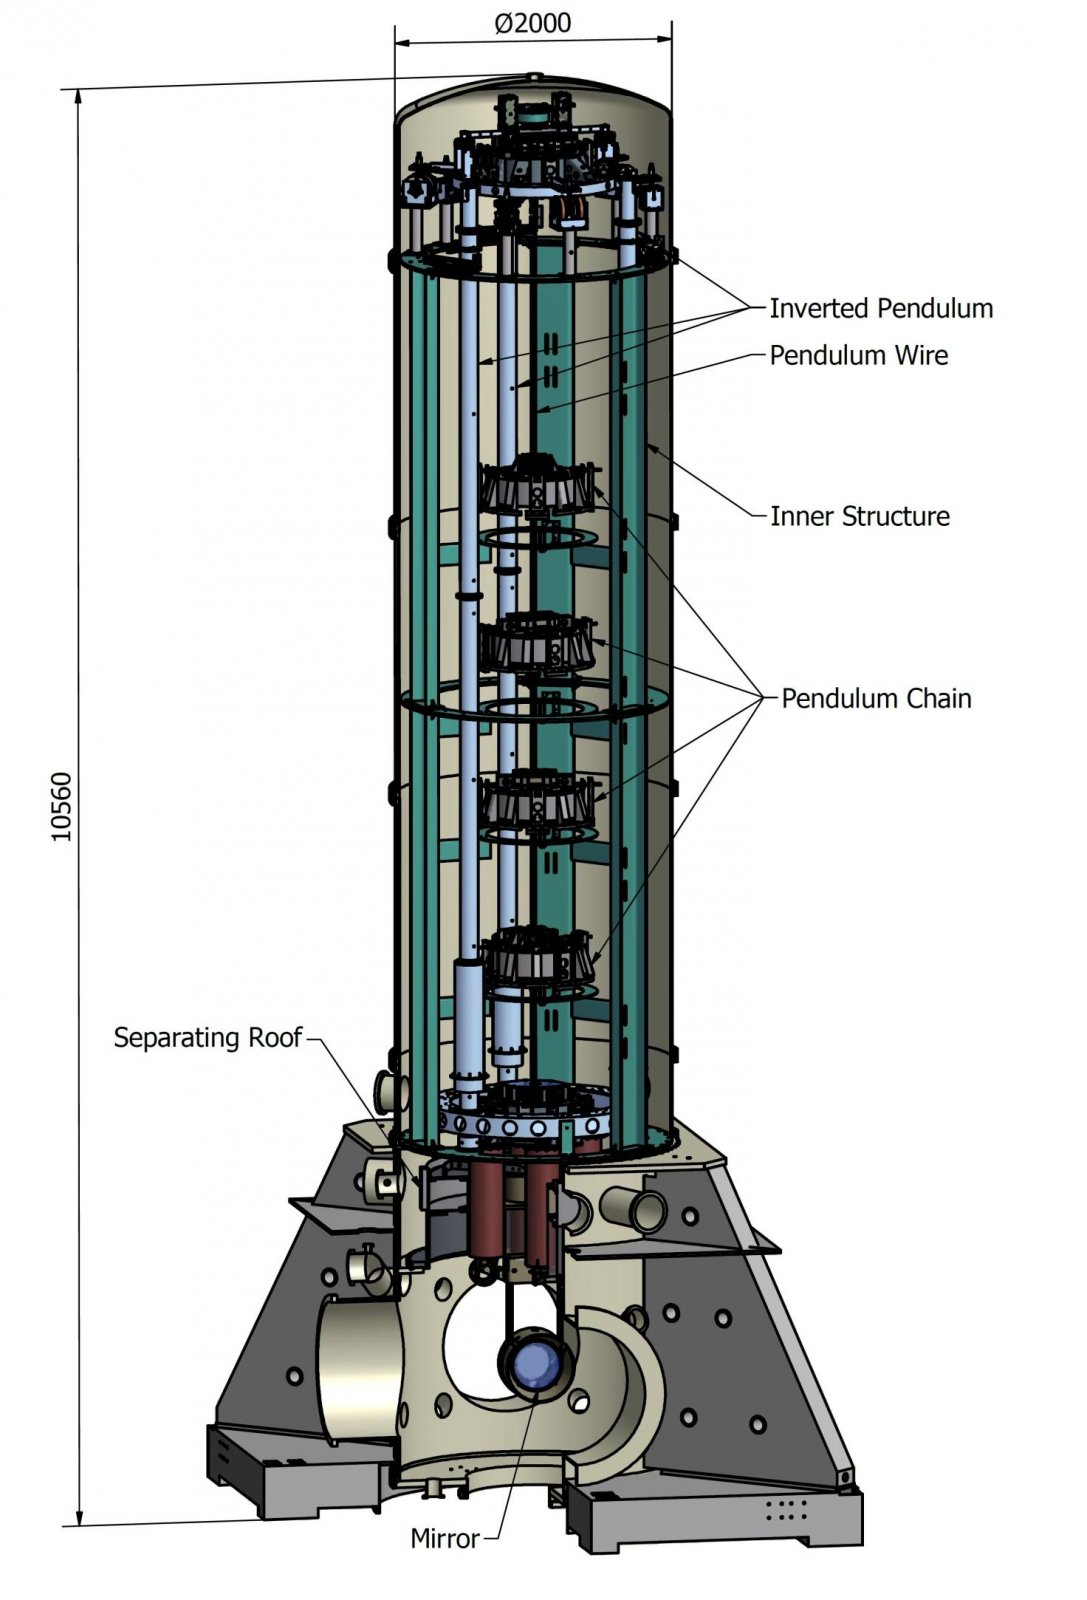
\includegraphics[width=0.5\textwidth]{superattenuator.jpg}
	\caption{\label{fig:superattenuator}
		A 3D model of the Virgo superattenuator (figure from \cite{Accadia_2012})}
\end{figure}

In a similar fashion as with LIGO, Virgo was also equipped with a number of incremental upgrades aimed at improving the sensitivity and testing the maturity of technologies needed for the subsequent version of the detector.
Most notably, the laser power was increased from 10\,W to 25\,W, a thermal compensation system was added, and the test masses were suspended using fused silica fibers directly bonded to the optics to reduce thermal noise\cite{Lorenzini_2010}.
In this configuration, the instrument was referred to as Virgo+.

\subsection{GEO 600 and other detectors}
GEO600~\cite{Grote_2010}, on the other hand, adopted quite different design choices, and pioneered a number of innovative technologies of which several would later be integrated in the larger detectors:
instead of Faby-P\'{e}rot arm cavities it employed folded arms, a topology in which the end of the arms are occupied by folding mirrors that send the laser back towards the end test masses located close to the beam splitter;
it was the first detector to employ a signal recycling cavity to shape the gravitational wave signal frequency response~\cite{Willke_2002};
it also employed DC readout, rather than the more conventional RF homodyne readout~\cite{DCreadout};
it was the first detector to use monolithic final-stage suspensions of the test-masses~\cite{Plissi_2000};
finally, it was the first to employ squeezing, a technique used to shape quantum fluctuations and obtain a reduction in relative shot noise equivalent to that of a higher power laser~\cite{Grote_2013}.
GEO600 was also the only observatory to remain active during the period in which LIGO and VIRGO were being upgraded to their second generation.
%TODO: reference figure in the text

\begin{figure}[htb]
	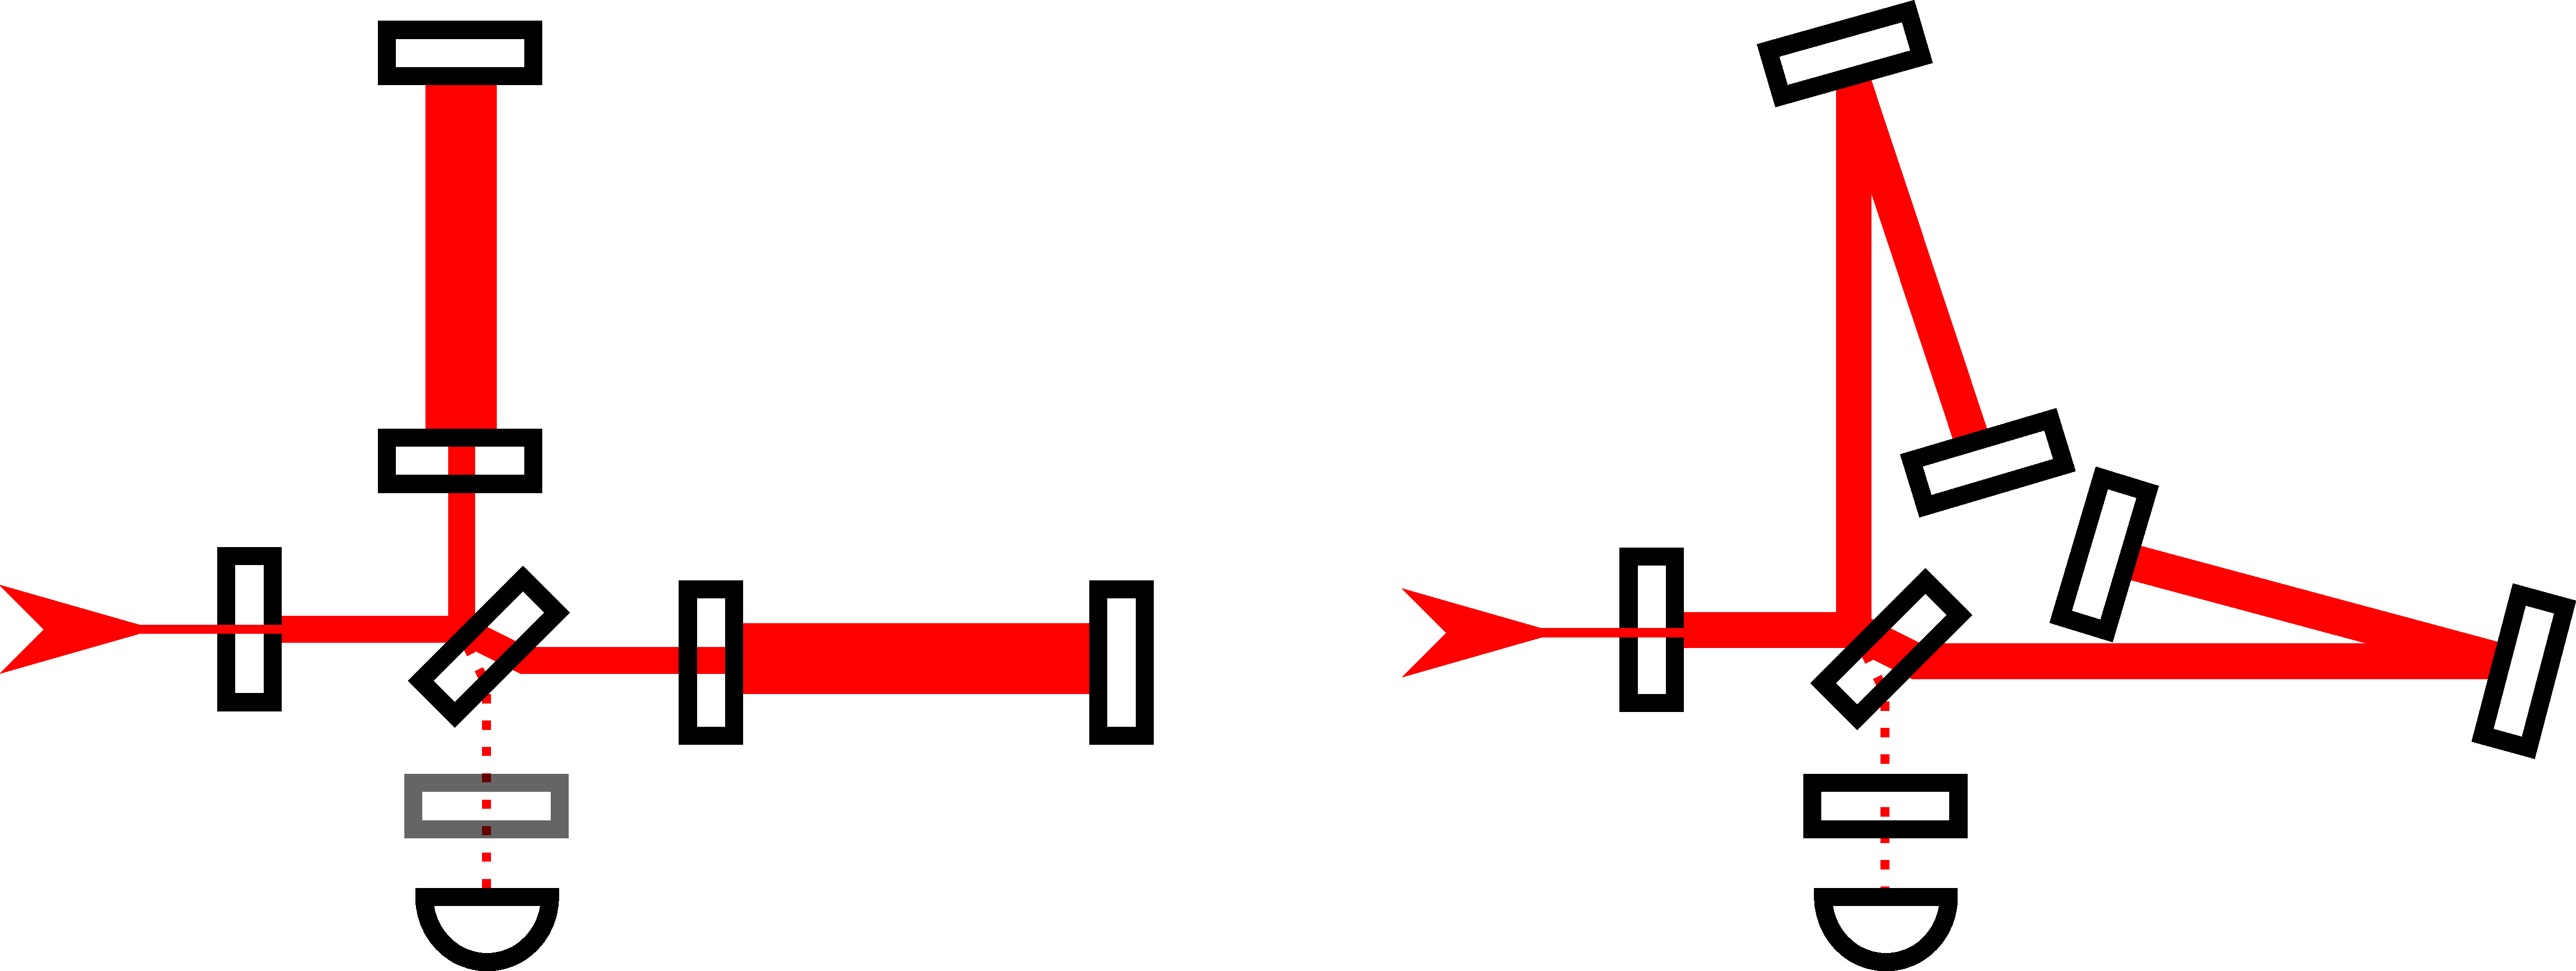
\includegraphics[width=\textwidth]{detector_layouts.pdf}
	\caption{\label{fig:detector_layouts}
		The optical layouts of the core interferometers of Advanced LIGO and Advanced Virgo (left), and GEO600 (right). 
		In the initial LIGO and Virgo detectors and TAMA300 the optical layout was as shown on the left, bar the omission of the 
signal recycling mirror, shown in the diagram in gray.}
\end{figure}

TAMA300\cite{Ando_2002}, in Japan, also adopted an optical layout similar to LIGO and VIRGO, although its smaller size and location in Tokyo severely limited its sensitivity below a few hundred Hz.
It nevertheless provided many useful results, including the development of sensing and control techniques that would be later transferred to the larger interferometers. 
The CLIO detector, also in Japan but situated in the Kamioka mine, began construction in 2003 and was eventually operated with cryogenically cooled test masses and demonstrated a reduced thermal noise level compared to room temperature~\cite{Uchiyama_2012}. However, with relatively short arm lengths of 100\,m CLIO could not come close to the strain sensitivities of the larger detectors.

\subsection{Looking for gravitational waves}
In 2002, the LIGO detectors and GEO600 reached a sensitivity adequate for collecting science data, although still far from the design goal.
The first science run took place between August and September 2002 with a conventional range (defined as the maximum distance at which an optimally oriented standard NS-NS coalescence could be detected with a signal-to-noise ratio equal to 8) of 100\,kpc; more than two orders of magnitude less than the design value of 18\,Mpc.
In the years that followed, LIGO conducted other 5 science runs, interrupted by commissioning periods that steadily and consistently improved the performance until it finally reached full design sensitivity in 2006.
In all but one of these science runs, the three LIGO detectors were run in coincidence with one or more other large scale detectors around the world (GEO600, Virgo and TAMA300) to leverage the superior noise rejection and sky localization capabilities of a widely distributed network of detectors\cite{Abbott_2004,Abbott_2005,Abbott_2006,Abbott_2008,Abadie_2010}.

%Approximate list of runs (including partners):
%2002: S1 (LIGO + GEO)
%2003: S2 LIGO + TAMA DT8)
%2004: S3 (LIGO)
%2005: S4 (LIGO + GEO)
%2005-2007: S5 (LIGO + GEO + VIRGO VSR1)
%2009-2010: S6 + VSR2-3